\documentclass[report]{subfiles}
\begin{document}
    \chapter{IMPLEMENTATION}
    \section {The main() function}
    The main function which can be found in the main.c file only calls the 3 important functions in the program i.e. \texttt{InitEverything()}, \texttt{MainProgramLoop()} and \texttt{CloseEverything}.
    \begin{lstlisting}
#include "program.h"

int main(int argc, char **argv)
{
    int grid[GRID_ROW * GRID_COL];
    //Initialize the window, char maps, grid, font, UI etc
    InitEverything(grid, argc, argv);
    //The main program loop. User input, drawing, output, simulation everything happens here
    MainProgramLoop(grid);
    //Destroying textures, window, renderer and closing fonts happens here
    CloseEverything();
    return 0;
}
    \end{lstlisting}
    \section{Initializing}
    Initializing consists of initializing the libraries, the grid, font and the character maps. Initializing is done through the \texttt{InitEverything()} function which calls other helper functions to prepare everything as shown below: 
    \begin{lstlisting}
TTF_Font *font = NULL;             //Font used in UI
TTF_Font *displayFont = NULL;      //Font used in decoders
SDL_Texture *characters[127 - 32]; //Character map for UI
int characterWidth[127 - 32];
SDL_Texture *displayChars[16]; //Character Map for decoders

void InitEverything(int grid[GRID_ROW * GRID_COL], int argc, char **argv)
{
    // Initialize SDL
    if (SDL_Init(SDL_INIT_EVERYTHING) < 0)
        exit(-1);
    // Create Window and renderer
    window = SDL_CreateWindow("MinimaLogic", 0, 0, WINDOW_WIDTH, WINDOW_HEIGHT, SDL_WINDOW_MAXIMIZED | SDL_WINDOW_RESIZABLE);
    renderer = SDL_CreateRenderer(window, -1, SDL_RENDERER_SOFTWARE);
    if (!(window && renderer))
        exit(-2);
    // Set minimum size for the window
    SDL_SetWindowMinimumSize(window, MIN_WINDOW_WIDTH, MIN_WINDOW_HEIGHT);
    // Initialize the grid
    InitGrid(grid);
    // If user clicked on a .mlg file and opened it with
    // Minimalogic.exe then read from that file and then update grid and window title
    if (argc > 1){
        ReadFromFile(grid, argv[1]);
        fileExists = true;
        SDL_strlcpy(currentFile, argv[1], 256);
        UpdateWindowTitle(argv[1]);
    }
    // Get width and height of the window
    int w, h;
    SDL_GetWindowSize(window, &w, &h);
    // Initialize the Menu
    InitMenu(w, h, false);
    //Change directory to location of the executable so that the program can find fonts
    char *path = argv[0], i;
    for (i = SDL_strlen(path) - 1; path[i] != '\\'; i--);
    path[i] = '\0';
    _chdir(path);
    // Initialize fonts
    InitFont();
    // Create character maps
    CharacterMap();
    // Close fonts and SDL_ttf since they are no longer needed
    TTF_CloseFont(font);
    TTF_CloseFont(displayFont);
    TTF_Quit();
}
    \end{lstlisting}
    \subsection{Initializing Menu}
    To initialize the menu, the \texttt{InitMenu()} function is called which sets positions and dimensions for all buttons in the menu. For the buttons, we have defined a Button struct as follows:
    \begin{lstlisting}
typedef struct Button
{
    SDL_Rect buttonRect;  // contains the position and dimension of the buttons
    Selection selection;
    SDL_Color color;      // holds the color of the button
} Button;
    \end{lstlisting}
    The \texttt{SDL\_Rect} and \texttt{SDL\_Color} are structs defined by SDL2. They have been discussed in the Rendering section. We have Selection the selection struct as shown below. It holds the information needed to place a component on the grid.
    \begin{lstlisting}
typedef struct
{
    Type type; //Type enum to store type of component
    char size; //size of the component
    Pair pos;  //position of the component
} Selection;
    \end{lstlisting}
    The Pair struct only stores a pair of integers.
    \begin{lstlisting}
typedef struct
{
    int x, y;
} Pair;
    \end{lstlisting}
    The \texttt{InitMenu()} function is defined as follows:
    \begin{lstlisting}
// Declare all buttons used in program as globals
Button confirmYes = {.color = {GREEN, 255}};
Button confirmNo = {.color = {RED, 255}};
Button confirmCancel = {.color = {BLUE, 255}};
Button Components[g_total];
Button SideMenu[sm_total];
Button FileMenu[fm_total];

void InitMenu(int windowWidth, int windowHeight, bool simulating)
{
    // Set color, position and dimension for all buttons in the side menu
    for (int i = 0; i < sm_total; i++)
    {
        SideMenu[i].buttonRect.w = MENU_WIDTH - 20;
        SideMenu[i].color = (SDL_Color){BLACK};
        SideMenu[i].buttonRect.h = MENU_FONT_SIZE;
        SideMenu[i].buttonRect.x = 10;
        SideMenu[i].buttonRect.y = windowHeight - (sm_total - i) * (10 + SideMenu[i].buttonRect.h);
    }
    // Set color, position and dimension for all buttons in the file menu
    for (int i = 0; i < fm_total; i++)
    {
        FileMenu[i].buttonRect.w = MENU_WIDTH - 20;
        FileMenu[i].buttonRect.h = MENU_FONT_SIZE;
        FileMenu[i].buttonRect.x = windowWidth / 2 - FileMenu[i].buttonRect.w / 2;
        FileMenu[i].buttonRect.y = windowHeight / 2 +
                                   FileMenu[i].buttonRect.h / 2 +
                                   (i - fm_total / 2) * (FileMenu[i].buttonRect.h + 10);
    }
    // Set color of the RUN/STOP button
    // also set its position to be at the top of the screen 
    if (simulating)
        SideMenu[sm_run].color = (SDL_Color){RED};
    else
        SideMenu[sm_run].color = (SDL_Color){GREEN};
    SideMenu[sm_run].buttonRect.y = 10;
    // Set Components (dropdown) button to be right below RUN/STOP button
    SideMenu[sm_compo].buttonRect.y = SideMenu[sm_run].buttonRect.y + SideMenu[sm_compo].buttonRect.h + 10;

    // Set color, dimension and position of the - (decrease inputs) button
    SideMenu[sm_dec].color = (SDL_Color){RED};
    SideMenu[sm_dec].buttonRect.w = 0.15 * MENU_WIDTH - 10;
    SideMenu[sm_dec].buttonRect.x = 10;

    // Set position and dimension for rect which shows no. of inputs of current choice
    InputsCount.x = SideMenu[sm_dec].buttonRect.x + SideMenu[sm_dec].buttonRect.w + 5;
    InputsCount.y = SideMenu[sm_dec].buttonRect.y;
    InputsCount.w = 0.7 * MENU_WIDTH - 10;
    InputsCount.h = MENU_FONT_SIZE;

    // Set color, dimension and position of the + (increase inputs) button
    SideMenu[sm_inc].color = (SDL_Color){RED};
    SideMenu[sm_inc].buttonRect.w = 0.15 * MENU_WIDTH - 10;
    SideMenu[sm_inc].buttonRect.x = InputsCount.x + InputsCount.w + 5;
    SideMenu[sm_inc].buttonRect.y = SideMenu[sm_dec].buttonRect.y;

    /* Buttons in the confirmation screen */
    confirmYes.buttonRect.w = 150;
    confirmYes.buttonRect.h = MENU_FONT_SIZE;
    confirmYes.buttonRect.x = windowWidth / 2 - 200 + 25;
    confirmYes.buttonRect.y = windowHeight / 2 - 100 + 200 - confirmYes.buttonRect.h - 15 - MENU_FONT_SIZE;

    confirmNo.buttonRect.w = 150;
    confirmNo.buttonRect.h = MENU_FONT_SIZE;
    confirmNo.buttonRect.x = windowWidth / 2 - 200 + 400 - 25 - confirmNo.buttonRect.w;
    confirmNo.buttonRect.y = windowHeight / 2 - 100 + 200 - confirmNo.buttonRect.h - 15 - MENU_FONT_SIZE;

    confirmCancel.buttonRect.w = 150;
    confirmCancel.buttonRect.h = MENU_FONT_SIZE;
    confirmCancel.buttonRect.x = windowWidth / 2 - confirmCancel.buttonRect.w / 2;
    confirmCancel.buttonRect.y = windowHeight / 2 - 100 + 200 - confirmCancel.buttonRect.h - 10;

    // Buttons in the dropdown
    for (int i = 0; i < g_total; i++)
    {
        Components[i].selection.type = i;
        Components[i].selection.size = 2;
        Components[i].buttonRect.x = 20;
        Components[i].buttonRect.y = SideMenu[sm_compo].buttonRect.y +
                                     SideMenu[sm_compo].buttonRect.h +
                                     i * (CELL_SIZE * SCALE + 2) + 10;
        Components[i].buttonRect.w = MENU_WIDTH - 40;
        Components[i].buttonRect.h = MENU_FONT_SIZE - 10;
    }
}
    \end{lstlisting}
    In the above function, all values starting with \texttt{sm\_} and \texttt{fm\_} are part of following enums:
    \begin{lstlisting}
// enum to keep track of buttons in the side menu
typedef enum {sm_run, sm_compo, sm_inc, sm_dec, sm_undo, sm_redo, sm_snap, sm_delete, sm_clear, sm_fmenu, sm_total } SidemenuButtons;
// enum to keep track of buttons in the file menu
typedef enum{ fm_new, fm_open, fm_save, fm_saveas, fm_exitm, fm_exitp, fm_total } FileMenuButtons;
    \end{lstlisting}
    These enums are also used later to check which button the user clicked.
    \subsection{Initializing the grid}
    Initializing the grid is a simple process, it only consists of filling the grid with -1 which represents empty space.
    \begin{lstlisting}
void InitGrid(int grid[GRID_ROW * GRID_COL])
{
    for (int i = 0; i < GRID_COL * GRID_ROW; i++)
        grid[i] = -1;
}
    \end{lstlisting}
    In case the user has opened a .mlg file using Minimalogic, the file will be read and the grid will be updated accordingly by the \texttt{ReadFromFile()} function which has been described later in User Interaction section.
    \subsection {Initializing fonts and Creating Character maps}
    In our program, we are rendering text by displaying a texture containing a character onto the screen. The process of creating a texture for a character and then displaying it to the screen is very heavy. So doing this every time we have to render text will be extermely inefficient. Thus to counter this, we create character maps once at the start of the program which can be used to render text later without having to create a texture everytime.
    \begin{lstlisting}
// function to initialize SDL_ttf and load fonts to be used
static void InitFont()
{
    TTF_Init(); // initialize sdl_ttf
    // load fonts
    font = TTF_OpenFont("ui_font.ttf", 25);
    displayFont = TTF_OpenFont("led_font.otf", 100);
    // exit program if loading fonts fails
    if (font == NULL || displayFont == NULL)
    {
        SDL_Log("Failed to load the font: %s\n", TTF_GetError());
        exit(-3);
    }
}
// function to create character maps
void CharacterMap()
{
    // list of all characters for decoders
    char *nums[16] = {"0", "1", "2", "3", "4", "5", "6", "7", "8", "9", "A", "B", "C", "D", "E", "F"};
    // surface to be used to create texture
    SDL_Surface *characterSurface;
    SDL_Color white = {WHITE, 200};
    SDL_Color black = {BLACK, 255};

    // create texture for characters having unicode (32 - 127)
    // this includes all characters of english alphabet as well as special symbols and numbers
    for (int i = 32; i < 127; i++)
    {
        // render character on surface
        characterSurface = TTF_RenderText_Blended(font, (char *)&i, white);
        // make texture from surface
        characters[i - 32] = SDL_CreateTextureFromSurface(renderer, characterSurface);
        // get width of the character (used to retain proper shape of character)
        characterWidth[i - 32] = characterSurface ? characterSurface->w : 0;
    }
    // similar process for characters to be shown in decoders
    for (int i = 0; i < 16; i++)
    {
        characterSurface = TTF_RenderText_Blended(displayFont, nums[i], black);
        displayChars[i] = SDL_CreateTextureFromSurface(renderer, characterSurface);
    }
    // free the surface to free memory
    SDL_FreeSurface(characterSurface);
}
    \end{lstlisting}
    \section{Main Program Loop}
    Everything the user sees and does happens in the main program loop. In our program this loop has been defined inside the \texttt{MainProgramLoop()} function. The outline of the loop has been given below:
    The particular steps in the loop have been explained in the following sections.
    \begin{figure}[H]
        \centering
        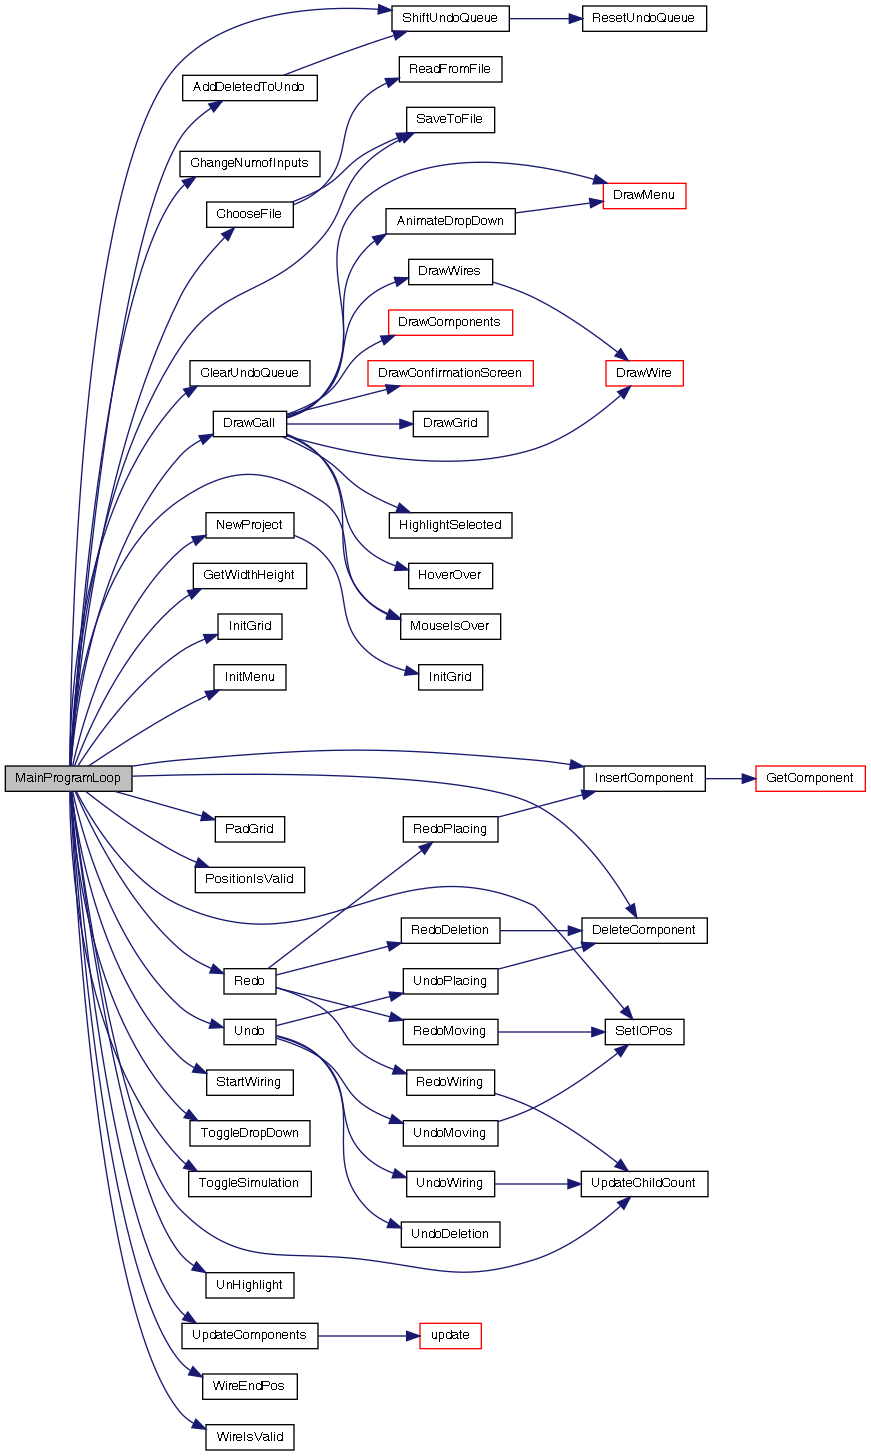
\includegraphics[height=\textheight]{../graphics/main_loop_call_tree.png}
        \caption{Call tree for MainProgramLoop}
    \end{figure}
    Code for the main program loop:
    \begin{lstlisting}
Actions UndoBuffer[MAX_UNDOS];
void MainProgramLoop(int grid[GRID_ROW * GRID_COL])
{
    // defining various fields required during the loop
    Selection compoChoice = {.type = 0, .size = 0};
    Pair selected = {-1, -1};

    int x, y;
    Pair gridPos;
    int pad_x, pad_y;
    PadGrid(&pad_x, &pad_y);

    int sender, receiver, sendIndex, receiveIndex, compoMoved;
    bool simulating = false, menuExpanded = false, drawingWire = false, movingCompo = false, confirmWire = false;
    bool snapToGrid = false, snapToggeled = false, cursorInGrid, draw, updated = false, ctrlHeld = false;
    char dropDownAnimationFlag = 0, startAt = 0, endAt = 0, animating = 8;
    Pair offset, initialPos;
    ConfirmationFlags confirmationScreenFlag = none;
    unsigned char updateOrder[256];

    int currentUndoLevel = 0, totalUndoLevel = 0;
    bool run = true;

    SDL_Event e;
    while (run)
    {
        // to make sure the program runs at consistent fps
        int begin = SDL_GetTicks();
        // to limit how many times drawing is done
        draw = !simulating;
        // get mouse cursor position
        SDL_GetMouseState(&x, &y);
        // get position of mouse relative to the grid
        if (x - pad_x > 0)
            gridPos.x = (x - pad_x) / CELL_SIZE;
        else
            gridPos.x = -1;
        if (y - pad_y > 0)
            gridPos.y = (y - pad_y) / CELL_SIZE;
        else
            gridPos.y = -1;
        // mod the position of mouse by SCALE/2 if snapping is toggled
        // this will make the component preview snap to half of the gridlines
        if (snapToGrid && gridPos.x >= 0 && gridPos.y >= 0)
        {
            gridPos.x -= gridPos.x % (SCALE / 2);
            gridPos.y -= gridPos.y % (SCALE / 2);
        }
        // check wheter cursor is in the grid or not
        cursorInGrid = gridPos.x >= 0 && gridPos.x < GRID_ROW && gridPos.y >= 0 &&
                       gridPos.y < GRID_COL;
        // getting and handling user input
        while (SDL_WaitEventTimeout(&e, DELAY / 10))
        {
             /* see User Interaction section */
             // Draw once and only if any updates occur
            if (draw)
            {
                DrawCall(menuExpanded, drawingWire, x, y, compoChoice, pad_x, pad_y,
                         simulating, &dropDownAnimationFlag, gridPos, grid, movingCompo, selected, snapToGrid, confirmationScreenFlag);
                draw = false;
            }
        }
        // updating components if simulation is running
        if (simulating)
        {
            for (int i = 0; i < 256; i++)
                AlreadyUpdated[i] = false;
            UpdateComponents(updateOrder);
            time += DELAY;
            if (time >= DELAY * 20)
                time = 0;
            selected = (Pair){-1, -1};
        }
        // Always draw if simulation is running or an animation is running
        if (simulating || animating < 8)
            DrawCall(menuExpanded, drawingWire, x, y, compoChoice, pad_x, pad_y,
                     simulating, &dropDownAnimationFlag, gridPos, grid, movingCompo, selected, snapToGrid, confirmationScreenFlag);
        // to keep track of the animation
        animating += 1;
        animating = (animating > 8)? 8 : animating;
        // Delay the loop to limit frame rate and redude load on cpu
        if ((SDL_GetTicks() - begin) < DELAY)
            SDL_Delay(DELAY - (SDL_GetTicks() - begin));
        else
            SDL_Delay(DELAY);
    }
}
\end{lstlisting}
In order to optimize our program and make it more efficient, we have tried to render/draw things as few times as possible. This has been obtained by rendering only if user provides some imput or the simulation or animation is running. Doing this dramatically lessens the load on the CPU.
\subsection{The Components}
To make the components we have defined a Component (\_component) struct as follows:
\begin{lstlisting}
typedef struct _component
{
    Pair start,         // position of the component on the grid
         inpPos[MAX_INPUTS],    // position of input terminals
         outPos[MAX_TERM_NUM],  // position of output terminals
         inpSrc[MAX_INPUTS];    // source for inputs array also used to make wires
    unsigned char size,     // height of the component
                  width,    // width of the component
                  inum,     // no. of inputs
                  onum,     // no. of outputs
                  childCount;    // no.of components which directly or indirectly get input from this component
    bool outputs[MAX_TERM_NUM];  // to keep track of outputs after updating
    Type type;      //Type of component
    struct _component *inputs[MAX_INPUTS];  //pointer to Components providing input
} Component;
\end{lstlisting}
By using an array of pointers to keep track of inputs,  we have applied a dort of backwards linked list approach which allows us to prevent errors while updating the components. The type of component is determined by the following enum:
\begin{lstlisting}
typedef enum{ state, probe, clock, g_not, d_oct, d_4x16, g_and, g_or, g_nand, g_nor, g_xor, g_xnor, g_total} Type;
\end{lstlisting}
\subsection{Updating A Component}
Updating a component is implemented in the following way: 
\begin{lstlisting}
// declaring function for each component
static void Tick(Component *component);
static void orGate(Component *component);
static void andGate(Component *component);
static void notGate(Component *component);
static void norGate(Component *component);
static void xorGate(Component *component);
static void xnorGate(Component *component);
static void nandGate(Component *component);
static void DoNothing(Component *component);
static void Decode(Component *component);
static int BinToDec(bool[4]);
// to keep track of components being updated and prevent infinite recursion
bool AlreadyUpdated[256];

// array of function pointers so that we can call appropriate function according to the type of component to update it
static void (*operate[g_total])(Component *component) = {DoNothing, DoNothing, Tick, notGate, Decode, Decode, andGate, orGate, nandGate, norGate, xorGate, xnorGate};

// function to update the components providing input
// by using the backwards linked list approach we first update the components providing input so that correct output can be produced
static void SetInputs(Component *component)
{
    for (int i = 0; i < component->inum; i++)
    {
        if (component->inpSrc[i].x != -1)
        {
            // to update component only once and prevent stack overflow via recursion
            if (!AlreadyUpdated[component->inpSrc[i].x])
            {
                AlreadyUpdated[component->inpSrc[i].x] = true;
                update(component->inputs[i]);
            }
        }
    }
}
// This function first calls the SetInputs() function and then calls appropriate function according to type of array
void update(Component *component)
{
    SetInputs(component);
    operate[component->type](component);
}

// function for and gate
static void andGate(Component *component)
{
    // set initial value if possible else set false as default value
    if (component->inpSrc[0].x >= 0){
        component->outputs[0] = component->inputs[0]->outputs[component->inpSrc[0].y];
    }
    else{
        component->outputs[0] = false;
    }
    // loop through all inputs and AND all of them to get output
    for (int i = 1; i < component->inum; i++){
        if (component->inpSrc[i].x >= 0){
            component->outputs[0] = component->outputs[0] && component->inputs[i]->outputs[component->inpSrc[i].y];
        }
        else{
            component->outputs[0] = false;
            break;
        }
    }
}
// other components work similarly
\end{lstlisting}
Here, the working of And gate has been described. Other gates are also updated similarly which can be seen in the full source code.
\subsection{Updating All Component}
As seen above, components placed on the grid only update if the simulation is running. Updating all the components happens through the \texttt{UpdateComponents()} function.
This function loop through the list of components and updates all of them once using the \texttt{update()} function shown above.
\begin{lstlisting}
static void UpdateComponents(unsigned char *updateOrder){
    for (int i = 0; i < componentCount; i++){
        unsigned char index = updateOrder[i];
        if (!AlreadyUpdated[index]){
            AlreadyUpdated[index] = true;
            update(&ComponentList[index]);
        }
    }
}
\end{lstlisting}
The \texttt{updateOrder} seen above is an array specifying the order in which the components should be updated. This is done to prevent jittering. The order is determining by sorting the components according to their \texttt{childCount}.
    \section{User Interaction}
    Getting and handling user interaction is the biggest portion of our program. This is done in a loop nested inside the main program loop. In this loop we wait for user input and then utilize \texttt{switch ... case} statements to respond to the inputs.
\begin{lstlisting}
// wait for user input
while (SDL_WaitEventTimeout(&e, DELAY / 10))
{
    switch (e.type)
    {
    // ask user if the want to save if they quit if they have made changes
    // else just set run to false which ends the main program loop
    case SDL_QUIT:
        if (fileExists && updated)
            confirmationScreenFlag = q_saveChanges;
        else if (updated && componentCount > 0)
            confirmationScreenFlag = q_saveNewFile;
        else
            run = false;
    case SDL_WINDOWEVENT:
    {
        // rearrange the grid and menu if window is resized
        int w, h;
        SDL_GetWindowSize(window, &w, &h);
        InitMenu(w, h, simulating);
        PadGrid(&pad_x, &pad_y);
        break;
    }
    case SDL_MOUSEBUTTONDOWN:
        // handling mouse clicks
        if (!confirmationScreenFlag)
        {
            // this code is executed only if no confirmation screen or menu is shown
            if (e.button.button == SDL_BUTTON_RIGHT)
            {
                selected = (Pair){-1, -1};
                break;
            }
            if (cursorInGrid)
            {
                if (!WireIsValid(grid, gridPos, x, y, pad_x, pad_y) && cell(gridPos.y, gridPos.x) >= 0)
                {
                    // this code is executed if user clicked on a component
                    // flip value of state and clock if they are clicked
                    if (ComponentList[cell(gridPos.y, gridPos.x)].type == state || (ComponentList[cell(gridPos.y, gridPos.x)].type == clock))
                        ComponentList[cell(gridPos.y, gridPos.x)].outputs[0] = !ComponentList[cell(gridPos.y, gridPos.x)].outputs[0];
                    if (!drawingWire && !movingCompo && !simulating)
                    {
                        // select component (used for deleting)
                        selected = gridPos;
                        // the following code is used to start move a placed component around on a grid
                        // which component?
                        Component compo = ComponentList[cell(gridPos.y, gridPos.x)];
                        // initial position of the component
                        initialPos = compo.start;
                        // offset from cursor to the topleft corner of component
                        offset = (Pair){gridPos.x - initialPos.x, gridPos.y - initialPos.y};
                        // which component?
                        compoMoved = cell(gridPos.y, gridPos.x);
                        // signify that we are moving a component now
                        movingCompo = true;
                        // empty the space being occupied by the component
                        for (int i = initialPos.y; i < initialPos.y + compo.size; i++)
                            for (int j = initialPos.x; j < initialPos.x + compo.width; j++)
                                cell(i, j) = -1;
                    }
                }
                else
                {
                    selected = (Pair){-1, -1};
                }
                // dimension of component user is trying to place
                int w, h;
                GetWidthHeight(&w, &h, compoChoice.type, compoChoice.size);
                // Check if component should be placed
                if (componentCount < 255 && !simulating && !drawingWire && PositionIsValid(grid, w, h, compoChoice.pos) && !movingCompo)
                {
                    // place the component
                    InsertComponent(grid, compoChoice, w, h);
                    // signify that an update has been made
                    updated = true;
                    // add this action to undo buffer so that it can be undoed
                    ShiftUndoBuffer(&currentUndoLevel, &totalUndoLevel);
                    UndoBuffer[0].act = 'p';
                    UndoBuffer[0].Action.placed.component = ComponentList[componentCount - 1];
                }
                else if (!simulating && !drawingWire && !movingCompo)
                {
                    // If user clicks on a terminal start drawing a wire
                    startAt = WireIsValid(grid, gridPos, x, y, pad_x, pad_y);
                    if (startAt < 0)
                    {
                        // wire begins at a output terminal
                        sender = cell(gridPos.y, gridPos.x);
                        sendIndex = startAt;
                        drawingWire = StartWiring((Pair){x, y});
                    }
                    else if (startAt > 0)
                    {
                        // wire begins at input terminal
                        receiver = cell(gridPos.y, gridPos.x);
                        receiveIndex = startAt;
                        drawingWire = StartWiring((Pair){x, y});
                    }
                }
            }
            // cursor is in the menu
            if (x <= MENU_WIDTH)
            {
                // which button was clicked
                Pair clickedButton = MouseIsOver(x, y, menuExpanded, compoChoice, confirmationScreenFlag == fileMenuFlag);
                if (clickedButton.x == sm)
                {
                    // button in side menu was clicked
                    if (clickedButton.y == sm_run)
                    {
                        // toggle simulation if RUN/STOP button is clicked
                        ToggleSimulation(&simulating, updateOrder);
                        selected = (Pair){-1, -1};
                    }
                    else if (!simulating)
                    {
                        // these buttons cant be clicked if simulation is running
                        switch (clickedButton.y)
                        {
                        case (sm_clear):
                            // clear button was clicked
                            // show confirmation screen
                            confirmationScreenFlag = clearGrid;
                            break;
                        case (sm_compo):
                            // component button was clicked
                            // toggle dropdown list
                            ToggleDropDown(&menuExpanded, &dropDownAnimationFlag);
                            animating = 0;
                            break;
                        case (sm_dec):
                            // decrease input if possible
                            ChangeNumofInputs(true, &compoChoice);
                            break;
                        case (sm_inc):
                            // increase input if possible
                            ChangeNumofInputs(false, &compoChoice);
                            break;
                        case (sm_delete):
                            // delete button clicked
                            // delete the selected component
                            // add the action to undo buffer
                            AddDeletedToUndo(&currentUndoLevel, &totalUndoLevel, cell(selected.y, selected.x));
                            DeleteComponent(grid, selected);
                            selected = (Pair){-1, -1};
                            updated = true;
                            break;
                        case (sm_undo):
                            // undo button clicked
                            // undo if possible
                            if (currentUndoLevel < totalUndoLevel)
                                Undo(grid, &currentUndoLevel, totalUndoLevel);
                            break;
                        case (sm_redo):
                            // redo button clicked
                            // redo if possible
                            if (currentUndoLevel > 0)
                                Redo(grid, &currentUndoLevel, totalUndoLevel);
                            break;
                        case (sm_snap):
                            // snap button clicked
                            // toggle snapping to grid
                            snapToGrid = !snapToGrid;
                            snapToggeled = !snapToggeled;
                            break;
                        case (sm_fmenu):
                            // open the file menu
                            confirmationScreenFlag = fileMenuFlag;
                            break;
                        default:
                            break;
                        }
                    }
                }
                else if (clickedButton.x == cm && menuExpanded)
                {
                    // one of the components in the dropdown component list was clicked
                    // update users choice of component to be place
                    UnHighlight(compoChoice.type);
                    compoChoice = Components[clickedButton.y].selection;
                }
            }
        }
        else
        {
            // a confirmation box or menu is shown
            Pair clickedButton = MouseIsOver(x, y, menuExpanded, compoChoice, confirmationScreenFlag == fileMenuFlag);
            char fname[256]; //name of file
            if (confirmationScreenFlag == fileMenuFlag && clickedButton.x == fm)
            {
                // file menu is open
                switch (clickedButton.y)
                {
                case fm_new:
                    // new button clicked
                    // ask to save if changes have been made
                    // then clear the grid for new project
                    if (fileExists && updated)
                        confirmationScreenFlag = n_saveChanges;
                    else if (updated && componentCount > 0)
                        confirmationScreenFlag = n_saveNewFile;
                    else
                    {
                        NewProject(grid, &updated);
                        confirmationScreenFlag = none;
                    }
                    break;
                case fm_open:
                    // open button clicked
                    // ask to save if changes have been made
                    // then open existing file
                    SDL_strlcpy(fname, currentFile, 256);
                    if (fileExists && updated)
                        confirmationScreenFlag = o_saveChanges;
                    else if (updated && componentCount > 0)
                        confirmationScreenFlag = o_saveNewFile;
                    else
                    {
                        ChooseFile(grid, false);
                        confirmationScreenFlag = none;
                    }
                    break;
                case fm_save:
                    // save button clicked
                    // save to file if it exists
                    // else make and save to new file
                    if (fileExists)
                        SaveToFile(grid, currentFile);
                    else
                        ChooseFile(grid, true);
                    updated = false;
                    confirmationScreenFlag = none;
                    break;
                case fm_saveas:
                    // save to a new file
                    ChooseFile(grid, true);
                    updated = false;
                    confirmationScreenFlag = none;
                    break;
                case fm_exitm:
                    // close the menu
                    confirmationScreenFlag = none;
                    break;
                case fm_exitp:
                    // exit program button clicked
                    // ask to save if changes have been made
                    // then set run to false
                    if (fileExists && updated)
                        confirmationScreenFlag = q_saveChanges;
                    else if (updated && componentCount > 0)
                        confirmationScreenFlag = q_saveNewFile;
                    else
                        run = false;
                    break;
                default:
                    break;
                }
            }
            else if (clickedButton.x == con && clickedButton.y > 0)
            {
                // confirmation screen and user clicked on yes
                switch (confirmationScreenFlag)
                {
                    // confirmation screen for what?
                case clearGrid:
                    // empty the grid
                    componentCount = 0;
                    InitGrid(grid);
                    updated = true;
                    break;
                case q_saveChanges:
                    // save changes on quitting
                    SaveToFile(grid, currentFile);
                    run = false;
                    break;
                case q_saveNewFile:
                    // save changes to new file on quitting
                    ChooseFile(grid, true);
                    run = false;
                    break;
                case o_saveChanges:
                    // save changes on opening existing file
                    SaveToFile(grid, currentFile);
                    ChooseFile(grid, false);
                    if (SDL_strcmp(fname, currentFile))
                    {
                        ClearUndoBuffer(&currentUndoLevel, &totalUndoLevel);
                        updated = false;
                    }
                    break;
                case o_saveNewFile:
                    // save changes to new file on opening existing file
                    ChooseFile(grid, true);
                    ChooseFile(grid, false);
                    if (SDL_strcmp(fname, currentFile))
                    {
                        ClearUndoBuffer(&currentUndoLevel, &totalUndoLevel);
                        updated = false;
                    }
                    break;
                case n_saveChanges:
                    // save changes on new file
                    SaveToFile(grid, currentFile);
                    NewProject(grid, &updated);
                    ClearUndoBuffer(&currentUndoLevel, &totalUndoLevel);
                    updated = false;
                    break;
                case n_saveNewFile:
                    // save changes to new file on new file
                    ChooseFile(grid, true);
                    NewProject(grid, &updated);
                    ClearUndoBuffer(&currentUndoLevel, &totalUndoLevel);
                    updated = false;
                    break;
                default:
                    break;
                }
                //close confirmation screen
                confirmationScreenFlag = none;
            }
            else if (clickedButton.x == con && !clickedButton.y)
            {
                // confirmation screen and user clicked on no
                // similar to when yes is clicked but no changes will be saved
                if (confirmationScreenFlag == q_saveChanges || confirmationScreenFlag == q_saveNewFile)
                    run = false;
                else if (confirmationScreenFlag == o_saveChanges || confirmationScreenFlag == o_saveNewFile)
                {
                    ChooseFile(grid, false);
                    if (SDL_strcmp(fname, currentFile))
                    {
                        updated = false;
                        ClearUndoBuffer(&currentUndoLevel, &totalUndoLevel);
                    }
                }
                else if (confirmationScreenFlag == n_saveChanges || confirmationScreenFlag == n_saveNewFile)
                {
                    NewProject(grid, &updated);
                    updated = false;
                    ClearUndoBuffer(&currentUndoLevel, &totalUndoLevel);
                }
                confirmationScreenFlag = none;
            }
            else if (clickedButton.x == con)
                confirmationScreenFlag = none;
        }
        break;
    case SDL_MOUSEBUTTONUP:
        // user stopped pressing mouse button
        if (drawingWire)
        {
            //if user was drawing wire 
            // check if wire can end where user left holding the mouse button
            endAt = WireIsValid(grid, gridPos, x, y, pad_x, pad_y);
            if (endAt && startAt != endAt)
            {
                // starting and ending component should not be same
                if (endAt < 0 && startAt > 0)
                {
                    // wire starts at input and ends at output terminal
                    sender = cell(gridPos.y, gridPos.x);
                    sendIndex = endAt;
                    confirmWire = true;
                }
                else if (endAt > 0 && startAt < 0)
                {
                    // wire starts at output and ends at input terminal
                    receiver = cell(gridPos.y, gridPos.x);
                    receiveIndex = endAt;
                    confirmWire = true;
                }
                if (sender != receiver && confirmWire)
                {
                    // wire can be made
                    // update the childcount for sender
                    // update inpSrc and input for receiver
                    if (ComponentList[receiver].inpSrc[receiveIndex - 1].x != -1)
                        UpdateChildCount(sender, false);
                    ComponentList[receiver].inpSrc[receiveIndex - 1] = (Pair){sender, sendIndex * -1 - 1};
                    ComponentList[receiver].inputs[receiveIndex - 1] = &ComponentList[sender];
                    updated = true;
                    for (int i = 0; i < 256; i++)
                        AlreadyUpdated[i] = false;
                    // Add this action to the undo buffer
                    UpdateChildCount(sender, true);
                    ShiftUndoBuffer(&currentUndoLevel, &totalUndoLevel);
                    UndoBuffer[0].act = 'w';
                    UndoBuffer[0].Action.wired.sender = sender;
                    UndoBuffer[0].Action.wired.connection.receiver = receiver;
                    UndoBuffer[0].Action.wired.connection.receiveIndex = receiveIndex - 1;
                    UndoBuffer[0].Action.wired.connection.sendIndex = sendIndex * -1 - 1;
                }
            }
            // stop drawing the wire
            drawingWire = false;
        }
        if (movingCompo)
        {
            // if a component was being moved
            Component compo = ComponentList[compoMoved];
            Pair finalPos = initialPos;
            if (compo.start.x < 0 || compo.start.y < 0)
            {
                // reset position of component if it goes outside the grid
                ComponentList[compoMoved].start = initialPos;
                SetIOPos(&ComponentList[compoMoved]);
            }
            if (!PositionIsValid(grid, compo.width, compo.size, compo.start))
            {
                // reset position of component if its position is invalid (overlapping)
                ComponentList[compoMoved].start = initialPos;
                SetIOPos(&ComponentList[compoMoved]);
            }
            else
                finalPos = compo.start; // give the component a new position if position is valid
            // update the grid
            for (int i = finalPos.y; i < finalPos.y + compo.size; i++)
                for (int j = finalPos.x; j < finalPos.x + compo.width; j++)
                    cell(i, j) = compoMoved;
            // no longer moving a component
            movingCompo = false;
            selected = finalPos;
            // add action to undo buffer if fincal and initial components are not same
            if (initialPos.x != compo.start.x || initialPos.y != compo.start.y)
            {
                updated = true;
                ShiftUndoBuffer(&currentUndoLevel, &totalUndoLevel);
                UndoBuffer[0].act = 'm';
                UndoBuffer[0].Action.moved.before = initialPos;
                UndoBuffer[0].Action.moved.after = finalPos;
                UndoBuffer[0].Action.moved.index = compoMoved;
            }
        }
    case SDL_MOUSEMOTION:
    {
        // get width and height of user's choice of component
        int w, h;
        GetWidthHeight(&w, &h, compoChoice.type, compoChoice.size);
        compoChoice.pos = gridPos;
        if (compoChoice.pos.x + w >= GRID_ROW)
            compoChoice.pos.x = GRID_ROW - w;
        if (compoChoice.pos.y + h >= GRID_COL)
            compoChoice.pos.y = GRID_COL - h;
    }
        if (drawingWire)
        {
            // update ending position of wire
            WireEndPos(x, y);
        }
        if (movingCompo)
        {
            // update position of component being moved
            Component compo = ComponentList[compoMoved];
            Pair newPos = {gridPos.x - offset.x, gridPos.y - offset.y};
            if (gridPos.x - offset.x + compo.width >= GRID_ROW)
                newPos.x = GRID_ROW - compo.width;
            if (gridPos.y - offset.y + compo.size >= GRID_COL)
                newPos.y = GRID_COL - compo.size;
            if (snapToGrid)
            {
                newPos.x -= newPos.x % (SCALE / 2);
                newPos.y -= newPos.y % (SCALE / 2);
            }
            newPos.x = newPos.x < 0 ? 0 : newPos.x;
            newPos.y = newPos.y < 0 ? 0 : newPos.y;

            compo.start = newPos;
            CollisionCheck(grid, &compo);
            ComponentList[compoMoved].start = compo.start;
            SetIOPos(&ComponentList[compoMoved]);
        }
        break;
    case SDL_KEYDOWN:
        // handling key pressess
        // these are just shortcuts for the buttons
        switch (e.key.keysym.scancode)
        {
        case SDL_SCANCODE_MINUS:
            ChangeNumofInputs(true, &compoChoice);
            break;
        case SDL_SCANCODE_EQUALS:
            ChangeNumofInputs(false, &compoChoice);
            break;
        case SDL_SCANCODE_DELETE:
            if (!simulating)
            {
                if (cursorInGrid && cell(gridPos.y, gridPos.x) >= 0)
                {
                    AddDeletedToUndo(&currentUndoLevel, &totalUndoLevel, cell(gridPos.y, gridPos.x));
                    DeleteComponent(grid, gridPos);
                    updated = true;
                }
                else if (selected.x >= 0)
                {
                    AddDeletedToUndo(&currentUndoLevel, &totalUndoLevel, cell(selected.y, selected.x));
                    DeleteComponent(grid, selected);
                    updated = true;
                }
                selected = (Pair){-1, -1};
            }
            break;
        case SDL_SCANCODE_LSHIFT:
            if (!snapToggeled)
                snapToGrid = true;
            break;
        case SDL_SCANCODE_RSHIFT:
            if (!snapToggeled)
                snapToGrid = true;
            break;
        case SDL_SCANCODE_LCTRL:
            ctrlHeld = !simulating;
            break;
        case SDL_SCANCODE_RCTRL:
            ctrlHeld = !simulating;
            break;
        case SDL_SCANCODE_Z:
            if (ctrlHeld && currentUndoLevel < totalUndoLevel)
                Undo(grid, &currentUndoLevel, totalUndoLevel);
            break;
        case SDL_SCANCODE_R:
            if (ctrlHeld && currentUndoLevel > 0)
                Redo(grid, &currentUndoLevel, totalUndoLevel);
            break;
        case SDL_SCANCODE_S:
            if (ctrlHeld)
            {
                if (fileExists)
                    SaveToFile(grid, currentFile);
                else
                    ChooseFile(grid, true);
                updated = false;
            }
            break;
        case SDL_SCANCODE_O:
            if (ctrlHeld && !simulating)
            {
                if (fileExists && updated)
                    confirmationScreenFlag = o_saveChanges;
                else if (updated && componentCount > 0)
                    confirmationScreenFlag = o_saveNewFile;
                else
                    ChooseFile(grid, false);
                ClearUndoBuffer(&currentUndoLevel, &totalUndoLevel);
                updated = false;
            }
            break;
        default:
            break;
        }
        break;
    case SDL_KEYUP:
        switch (e.key.keysym.scancode)
        {
        case SDL_SCANCODE_LSHIFT:
            snapToGrid = snapToggeled;
            break;
        case SDL_SCANCODE_RSHIFT:
            snapToGrid = snapToggeled;
            break;
        case SDL_SCANCODE_LCTRL:
            ctrlHeld = false;
            break;
        case SDL_SCANCODE_RCTRL:
            ctrlHeld = false;
            break;
        default:
            break;
        }
        break;
    default:
        break;
    }
    /* draw */
}
\end{lstlisting}
\subsection{Placing The Components}
Placing is done by following function. It gets an appropriate component according to the users choice and adds the component to the component list and updated the grid.
\begin{lstlisting}
// macro to make indexing grid easier
#define cell(y, x) grid[y * GRID_ROW + x]
//These are helper functions which set the values for membersoof component struct as per users choice
static Component MultiInputComponent(Type type, int inpNum, Pair pos)
{
    Component component;
    component.start = pos;
    component.size = inpNum;
    component.inum = inpNum;
    component.onum = 1;
    component.width = 4;
    component.size *= SCALE;
    component.width *= SCALE;
    component.childCount = 0;
    component.type = type;
    ClearIO(&component);
    SetIOPos(&component);
    return component;
}
static Component SingleInputComponent(Type type, Pair pos);
static Component MultiOutComponent(Type type, Pair pos);

// call appropriate helper function to match user choice
Component GetComponent(Type type, char inpNum, Pair pos)
{
    if (type <= g_not)
        return SingleInputComponent(type, pos);
    else if (type < g_and)
        return MultiOutComponent(type, pos);
    else
        return MultiInputComponent(type, inpNum, pos);
}

// update the list and the grid
void InsertComponent(int *grid, Selection choice, int width, int height)
{
    ComponentList[componentCount] =
        GetComponent(choice.type, choice.size, choice.pos);
    for (int y = choice.pos.y; y < choice.pos.y + height; y++)
    {
        for (int x = choice.pos.x; x < choice.pos.x + width; x++)
        {
            cell(y, x) = componentCount;
        }
    }
    componentCount++;
}
\end{lstlisting}
\subsection{Deleting a component}
Deleting a component is done by the following function:
\begin{lstlisting}
void DeleteComponent(int *grid, Pair gridPos)
{
    if (cell(gridPos.y, gridPos.x) == -1 || gridPos.x < 0 || gridPos.y < 0)
        return;
    // delete which component?
    int toDelete = cell(gridPos.y, gridPos.x);
    // empty the space occupied by that component in grid
    // decrease index of components whose index was higher than the one being deleted
    for (int i = 0; i < GRID_COL; i++)
    {
        for (int j = 0; j < GRID_ROW; j++)
        {
            if (cell(i, j) == toDelete)
                cell(i, j) = -1;
            else if (cell(i, j) > toDelete)
                cell(i, j)--;
        }
    }
    // if a component was getting input from the deleted component then set its imput source to empty
    // update input source of components whose inputs had index higher than the one being deleted
    for (int i = 0; i < componentCount; i++)
    {
        Component *compo = &ComponentList[i];
        for (int j = 0; j < compo->inum; j++)
        {
            if (compo->inpSrc[j].x == toDelete)
            {
                compo->inpSrc[j] = (Pair){-1, -1};
                compo->inputs[j] = NULL;
            }
            else if (compo->inpSrc[j].x > toDelete)
            {
                compo->inpSrc[j].x--;
                compo->inputs[j] = &ComponentList[compo->inpSrc[j].x];
            }
        }
    }
    // shift all the components having index higher than the one deleted forward in the list
    for (int i = toDelete; i < componentCount - 1; i++)
    {
        ComponentList[i] = ComponentList[i + 1];
    }
    componentCount--;
}
\end{lstlisting}
\subsection{Undo \& Redo}
Undo and Redo both rely on the undo buffer. Every time an action is taken, the changes made by it get pushed to the start of the buffer. This can be seen in the User Interaction code.
To keep track of the actions we have defined a seperate struct for each as follows:
\begin{lstlisting}
typedef struct
{
    unsigned char sendIndex, receiver, receiveIndex;
} Connection;

typedef struct
{
    unsigned char index, conNo;
    Component deletedCompo;
    Connection connections[255];
} Delete;

typedef struct
{
    unsigned char sender;
    Connection connection;
} Wiring;
typedef struct
{
    Component component;
} Place;

typedef struct
{
    unsigned char index;
    Pair before, after;
} Move;

typedef struct
{
    char act;
    union
    {
        Delete deleted;
        Wiring wired;
        Place placed;
        Move moved;
    } Action;
} Actions;
\end{lstlisting}
A union has been defined in the Actions struct so that only one type of action may be represented and to make it more memory efficient.

Everytime we undo, we first undo the action and then move forwards in the undo buffer i.e. "backwards in time". The \texttt{Undo} function undos the changes at current index in the undo buffer and moves forward in the buffer(index increases). A seperate helper function has been defined to undo each type of action.
Depending on the type of action appropriate helper function is called.
\begin{lstlisting}
static void UndoDeletion(Delete deleted, int *grid)
{
    int toDelete = deleted.index;

    for (int i = 0; i < GRID_COL; i++)
    {
        for (int j = 0; j < GRID_ROW; j++)
        {
            if (cell(i, j) >= deleted.index)
                cell(i, j)++;
        }
    }
    componentCount++;

    for (int i = 0; i < componentCount; i++)
    {
        Component *compo = &ComponentList[i];
        for (int j = 0; j < compo->inum; j++)
        {
            if (compo->inpSrc[j].x >= toDelete)
            {
                compo->inpSrc[j].x++;
                compo->inputs[j] = &ComponentList[compo->inpSrc[j].x];
            }
        }
    }
    for (int i = componentCount; i > deleted.index; i--)
    {
        ComponentList[i] = ComponentList[i - 1];
    }

    for (int i = 0; i < deleted.conNo; i++)
    {
        ComponentList[deleted.connections[i].receiver].inpSrc[deleted.connections[i].receiveIndex] = (Pair){deleted.index, deleted.connections[i].sendIndex};
        ComponentList[deleted.connections[i].receiver].inputs[deleted.connections[i].receiveIndex] = &ComponentList[deleted.index];
    }
    ComponentList[deleted.index] = deleted.deletedCompo;
    for (int i = deleted.deletedCompo.start.x; i < deleted.deletedCompo.start.x + deleted.deletedCompo.width; i++)
    {
        for (int j = deleted.deletedCompo.start.y; j < deleted.deletedCompo.start.y + deleted.deletedCompo.size; j++)
        {
            cell(j, i) = deleted.index;
        }
    }
}

static void UndoWiring(Wiring wired)
{
    for (int i = 0; i < 256; i++)
        AlreadyUpdated[i] = false;
    UpdateChildCount(wired.sender, false);
    ComponentList[wired.connection.receiver]
        .inpSrc[wired.connection.receiveIndex] = (Pair){-1, -1};
    ComponentList[wired.connection.receiver].inputs[wired.connection.receiveIndex] = NULL;
}

static void UndoPlacing(Place placed, int *grid)
{
    DeleteComponent(grid, placed.component.start);
}

static void UndoMoving(Move moved, int *grid)
{
    Component compo = ComponentList[moved.index];
    for (int i = moved.after.x; i < moved.after.x + compo.width; i++)
        for (int j = moved.after.y; j < moved.after.y + compo.size; j++)
            cell(j, i) = -1;
    for (int i = moved.before.x; i < moved.before.x + compo.width; i++)
        for (int j = moved.before.y; j < moved.before.y + compo.size; j++)
            cell(j, i) = moved.index;
    ComponentList[moved.index].start = moved.before;
    SetIOPos(&ComponentList[moved.index]);
}

void Undo(int *grid, int *currentUndoLevel, int totalUndoLevel)
{
    if (*currentUndoLevel >= totalUndoLevel)
        return;
    Actions toUndo = UndoBuffer[*currentUndoLevel];
    switch (toUndo.act)
    {
    case 'd':
        UndoDeletion(toUndo.Action.deleted, grid);
        break;
    case 'w':
        UndoWiring(toUndo.Action.wired);
        break;
    case 'p':
        UndoPlacing(toUndo.Action.placed, grid);
        break;
    case 'm':
        UndoMoving(toUndo.Action.moved, grid);
        break;
    default:
        break;
    }
    *currentUndoLevel += 1;
}
\end{lstlisting}
Redo is also done similarly except that we first move backwards in the undo buffer (index decreases) and then redo the action using a suitable helper function.
\begin{lstlisting}
static void RedoDeletion(Delete deleted, int *grid)
{
    DeleteComponent(grid, deleted.deletedCompo.start);
}

static void RedoWiring(Wiring wired)
{
    for (int i = 0; i < 256; i++)
        AlreadyUpdated[i] = false;
    UpdateChildCount(wired.sender, true);
    ComponentList[wired.connection.receiver].inpSrc[wired.connection.receiveIndex] = (Pair){wired.sender, wired.connection.sendIndex};
    ComponentList[wired.connection.receiver].inputs[wired.connection.receiveIndex] = &ComponentList[wired.sender];
}

static void RedoPlacing(Place placed, int *grid)
{
    Selection placing = {.type = placed.component.type, .size = placed.component.inum, .pos = placed.component.start};
    InsertComponent(grid, placing, placed.component.width, placed.component.size);
}

static void RedoMoving(Move moved, int *grid)
{
    Component compo = ComponentList[moved.index];
    for (int i = moved.before.x; i < moved.before.x + compo.width; i++)
        for (int j = moved.before.y; j < moved.before.y + compo.size; j++)
            cell(j, i) = -1;
    for (int i = moved.after.x; i < moved.after.x + compo.width; i++)
        for (int j = moved.after.y; j < moved.after.y + compo.size; j++)
            cell(j, i) = moved.index;
    ComponentList[moved.index].start = moved.after;
    SetIOPos(&ComponentList[moved.index]);
}

void Redo(int *grid, int *currentUndoLevel, int totalUndoLevel)
{
    *currentUndoLevel -= 1;
    Actions toRedo = UndoBuffer[*currentUndoLevel];
    switch (toRedo.act)
    {
    case 'd':
        RedoDeletion(toRedo.Action.deleted, grid);
        break;
    case 'w':
        RedoWiring(toRedo.Action.wired);
        break;
    case 'p':
        RedoPlacing(toRedo.Action.placed, grid);
        break;
    case 'm':
        RedoMoving(toRedo.Action.moved, grid);
        break;
    default:
        break;
    }
}
\end{lstlisting}
\subsection{Opening / Saving a file}
Opening and Saving file are done by using the \texttt{fwrite} and \texttt{fread} function provided by the \texttt{stdio.h} header.
To make this prosess easier for the user we have used the Windows API to open a dialog boc for the user in which they can open an existing file or create a file to save to.
\begin{lstlisting}
void ReadFromFile(int *grid, char *fileName)
{
    FILE *data = fopen(fileName, "rb");

    fread(&componentCount, sizeof(unsigned char), 1, data);
    fread(ComponentList, sizeof(Component), componentCount, data);
    fread(grid, sizeof(int), GRID_COL * GRID_ROW, data);

    for (int i = 0; i < componentCount; i++)
    {
        for (int j = 0; j < ComponentList[i].inum; j++)
        {
            ComponentList[i].inputs[j] = &ComponentList[ComponentList[i].inpSrc[j].x];
        }
    }

    fclose(data);
}

void SaveToFile(int *grid, char *fileName)
{
    FILE *data = fopen(fileName, "wb");
    fwrite(&componentCount, sizeof(unsigned char), 1, data);
    for (int i = 0; i < componentCount; i++)
    {
        fwrite(&ComponentList[i], sizeof(Component), 1, data);
    }
    for (int i = 0; i < GRID_ROW * GRID_COL; i++)
    {
        fwrite(&grid[i], sizeof(int), 1, data);
    }
    fclose(data);
}

void UpdateWindowTitle(char *FileName){
    char size = 0;
    char count = 0;
    char name[50] = "";
    while (FileName[size] != '\0')
    {
        if (FileName[size] == '\\')
            count = 0;
        name[count] = FileName[size + 1];
        count++;
        size++;
    }

    char title[70] = "MinimaLogic";
    SDL_strlcat(title, "-", 70);
    SDL_strlcat(title, name, 70);
    SDL_SetWindowTitle(window, title);

}

void ChooseFile(int *grid, bool saving)
{
    char FileName[256] = "";

    SDL_SysWMinfo wmInfo;
    SDL_VERSION(&wmInfo.version);
    SDL_GetWindowWMInfo(window, &wmInfo);

    OPENFILENAME ofn;
    memset(&ofn, 0, sizeof(ofn));
    ofn.lStructSize = sizeof(ofn);
    ofn.hwndOwner = wmInfo.info.win.window;
    ofn.hInstance = NULL;
    ofn.lpstrFilter = "Project Files (*.mlg)\0*.mlg";
    ofn.lpstrFile = FileName;
    ofn.nMaxFile = MAX_PATH;
    ofn.lpstrTitle = saving ? "Save File" : "Open File";
    ofn.lpstrDefExt = "mlg";
    ofn.Flags = OFN_NONETWORKBUTTON |
                OFN_FILEMUSTEXIST |
                OFN_HIDEREADONLY;
    if (!saving)
    {
        if (!GetOpenFileName(&ofn))
        {
            return;
        }
        else
        {
            ReadFromFile(grid, FileName);
            fileExists = true;
            SDL_strlcpy(currentFile, FileName, 256);
        }
    }
    else
    {
        if (!GetSaveFileName(&ofn))
        {
            return;
        }
        else
        {
            SaveToFile(grid, FileName);
            fileExists = true;
            SDL_strlcpy(currentFile, FileName, 256);
        }
    }
    UpdateWindowTitle(FileName);
}
\end{lstlisting}
    \section{Rendering}
    \textit{Note: Throughout this document, the words rendering and drawing have been used interchangeably}\\
    There are generally two ways to display graphic elements in an SDL window - displaying images using SDL surfaces or hardware rendering with textures and renderer. This program uses the later as the elements are too versatile to store them as bitmaps.
    \begin{figure}[H]
        \centering
        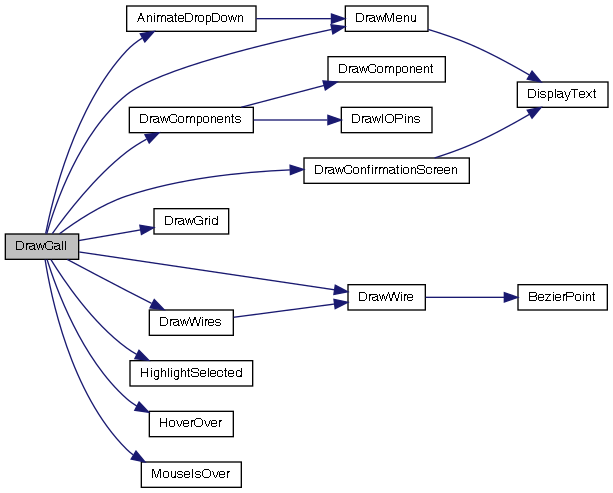
\includegraphics[width=0.5\textwidth]{../graphics/render_call_tree.png}
        \caption{Call tree for Rendering}
    \end{figure}
    For rendering all elements of the program, many functions have been called as shown in above figure. Most of these functions have been described below.
    \subsection{Functions for rendering in SDL}
    SDL provides a handful of functions which can be used to draw shapes such as lines, points, rectangles and filled rectangles. These shapes are very simple however the can be utilized to draw other complex shapes. But before we render a shape, we have to set its color.
    Each element on the screen may have a different color. So the renderer stores the color information when drawing anything on the screen. This information is stored if 4 channels commonly known as rgba format. The first three channels indicate intensity of red, green, and blue color respectively. The last channel is used to store the opaqueness of the element. The higher the value the higher the intensity. Before drawing an element on the screen, we must make sure that the renderer is set to the correct color value. This can be done using the function shown below.
\begin{lstlisting}
// SDL_SetRenderDrawColor(SDL_Renderer *, int red, green, blue, alpha);
SDL_SetRenderDrawColor(renderer, 255, 255, 255, 255);     //opaque white color
\end{lstlisting}
    \textbf{Rendering Lines}\\
    As mentioned previously, SDL provides direct functionality to draw a straight line between two points. The data doesn't need to be stored anywhere instead we can simply pass the co-ordinates of the points as parameters to the \texttt{SDL\_RenderDrawLine()} function and it will draw a line between those points for us. The co-ordinates are relative to the top left point of the window. This function has been used to draw the grid lines.
\begin{lstlisting}	
// SDL_RenderDrawLine(SDL_Renderer *, startX, startY, endX, endY);
SDL_SetRenderDrawLine(renderer, 0, 0, 50, 50);            //diagonal line form top left corner
\end{lstlisting}
To draw many lines at once, the \texttt{SDL\_RenderDrawLines()} function can be used which which takes an array of \texttt{SDL\_Point} and draws may lines by joining $n^{th}$ point in the array to the $(n + 1)^{th}$ point. This function has been used to draw wires joining the components.
\begin{lstlisting}	
SDL_RenderDrawLines(SDL_Renderer *, SDL_Point *array_of_points, int no_of_points);
\end{lstlisting}
    \textbf{Rendering Rectangles}\\
    In exchange for the low level access SDL provides, a lot of abstraction has been taken away. A rectangle is arguably the most complicated shape that can be drawn directly from the renderer in SDL. It can either be a rectangular outline or a solid rectangle filled with the current color configurations. In order to do so, the data for a rectangle must be stored using \texttt{SDL\_Rect} structure.
    \texttt{SDL\_Rect} structure has following members:
\begin{lstlisting}
    int x, y;    // coordinate of top left corner of the rectangle
    int w, h;    // width and height of the rectangle
\end{lstlisting}
The \texttt{SDL\_RenderDrawRect()} function can be used to render an outline of a rectangle and \texttt{SDL\_RenderFillRect()} function can be used to render a filled rectangle. Both of these functions take a \texttt{SDL\_Renderer *} and a \texttt{SDL\_Rect *} as parameters.
\begin{lstlisting}
SDL_Rect example = {10, 10, 200, 400};
SDL_SetRenderDrawColor(renderer, 255, 0, 0, 255);
//SDL_RenderDrawRect (SDL_Renderer *, SDL_Rect *);
SDL_RenderDrawRect (renderer, &example); // draws a red outline of a 200x400 px rectangle whose top left corner is at 10, 10
//SDL_RenderFillRect (SDL_Renderer *, SDL_Rect *);
SDL_RenderFillRect (renderer, &example); // draws a filled red 200x400 px rectangle whose top left corner is at 10, 10
\end{lstlisting}
The \texttt{SDL\_RenderDrawRect()} function has been used to draw highlight border around buttons and components. The \texttt{SDL\_FillRect()} has been heavily used to draw buttons, components, dialog boxes and menus.\\
In addition to these, \texttt{SDL\_RenderFillRects()} and \texttt{SDL\_RenderDrawRects()} are also available which can be used to draw multiple rectangles at once. We have used these functions to draw input/output terminals for the components.
\begin{lstlisting}	
SDL_RenderDrawRects(SDL_Renderer *, SDL_Rect *array_of_rect, int no_of_rects);
SDL_RenderFillRects(SDL_Renderer *, SDL_Rect *array_of_rect, int no_of_rects);
\end{lstlisting}
    \textbf{Rendering Text}\\
    As mentioned earlier, the text rendering is handled by an extension of the SDL library - SDL\_ttf. It provides the functionality to load ttf, rtf or otf fonts and create textures from them. An array of texture pointers is used to store the necessary ASCII characters. A texture is a structure that stores pixel data that can only be accessed through the GPU. Later, this array is used to display any message we want.
    In our program, we have implemented the text rendering as follows:\\
    \begin{lstlisting}
static void DisplayText(char *message, SDL_Rect parent){
    /* this function uses the character maps created
        during initialization to render certain text onto the screen */
    char *tmp = message;
    int totalWidth = 0; // total width of the message in pixels 
    float factor = 1; // factor to resize the text if it is too long
    // calculate total width
    for (; *tmp; tmp++)
        totalWidth += characterWidth[*tmp - 32];
    // rect onto which text will be rendered
    SDL_Rect charDest = {.y = parent.y, .h = parent.h};
    // calculate the factor
    if (totalWidth > parent.w){
        factor = parent.w / (float)totalWidth;
        tmp = message;
        totalWidth = 0;
        for (; *tmp; tmp++)
            totalWidth += characterWidth[*tmp - 32] * factor;
    }
    // center the text relative to the parent rect
    charDest.x = parent.x + (parent.w - totalWidth) / 2;
    // render each character in message onto the screen
    for (int i = 0; *message; message++, i++){
        charDest.w = characterWidth[*message - 32] * factor;
        SDL_RenderCopy(renderer, characters[*message - 32], NULL, &charDest);
        charDest.x += charDest.w;
    }
}
    \end{lstlisting}
	\subsection{Drawing the Menu}
\begin{lstlisting}
static void DrawMenu(bool menuExpanded, bool simulating, bool snap, Selection choice){
    // width, height of the window
    int w, h;
    SDL_GetWindowSize(window, &w, &h); 
    // background of menu
    SDL_Rect menuBg = {0, 0, MENU_WIDTH, h};
    SDL_SetRenderDrawColor(renderer, BG1); 
    SDL_RenderFillRect(renderer, &menuBg);
    // draw RUN/STOP button
    SDL_SetRenderDrawColor(renderer, SideMenu[sm_run].color.r, SideMenu[sm_run].color.g, SideMenu[sm_run].color.b, 255);
    SDL_RenderFillRect(renderer, &SideMenu[sm_run].buttonRect);
    if (simulating)
        DisplayText("STOP", SideMenu[sm_run].buttonRect);
    else
        DisplayText("RUN", SideMenu[sm_run].buttonRect);

    //draw all buttons in the side menu
    SDL_SetRenderDrawColor(renderer, SideMenu[sm_compo].color.r,  SideMenu[sm_compo].color.g, SideMenu[sm_compo].color.b, 255);
    for (int i = 1; i < sm_total; i++){
        if (i == sm_inc || i == sm_dec && choice.type < g_and)
            continue;
        SDL_RenderFillRect(renderer, &SideMenu[i].buttonRect);
        DisplayText(SideMenuButtonText[i], SideMenu[i].buttonRect);
    }

    if (snap)
        DisplayText("Snap to Grid: On", SideMenu[sm_snap].buttonRect);
    else
        DisplayText("Snap to Grid: Off", SideMenu[sm_snap].buttonRect);

    // draw buttons to inc/dec inputs and also display currnt no. of inputs
    if (choice.type >= g_and){
        SDL_SetRenderDrawColor(renderer, BLACK, 255);
        SDL_RenderFillRect(renderer, &InputsCount);
        char tmptxt[10] = "Inputs: ";
        tmptxt[8] = (char)(choice.size - 2 + 50);
        DisplayText(tmptxt, InputsCount);

        SDL_SetRenderDrawColor(renderer, SideMenu[sm_inc].color.r, SideMenu[sm_inc].color.g,
                               SideMenu[sm_inc].color.b, 255);
        SDL_RenderFillRect(renderer, &SideMenu[sm_inc].buttonRect);
        DisplayText("+", SideMenu[sm_inc].buttonRect);
        SDL_RenderFillRect(renderer, &SideMenu[sm_dec].buttonRect);
        DisplayText("-", SideMenu[sm_dec].buttonRect);
    }

    if (menuExpanded){
        SDL_Rect wrapper = {SideMenu[sm_compo].buttonRect.x,
                            SideMenu[sm_compo].buttonRect.y +
                            SideMenu[sm_compo].buttonRect.h,
                            SideMenu[sm_compo].buttonRect.w, 2 + g_total * (25 + 2)};
        SDL_SetRenderDrawColor(renderer, BG2);
        SDL_RenderFillRect(renderer, &wrapper);

        for (int i = 0; i < g_total; i++){
            SDL_SetRenderDrawColor(renderer, Components[i].color.r,
                                   Components[i].color.g, Components[i].color.b, 255);
            SDL_RenderFillRect(renderer, &Components[i].buttonRect);
            DisplayText(compoTexts[i], Components[i].buttonRect);
        }
    }
}
\end{lstlisting}
	\subsection{Drawing the Grid}
\begin{lstlisting}
static void DrawGrid(int pad_x, int pad_y){
    SDL_SetRenderDrawColor(renderer, BG2);
    for (int x = 0; x <= GRID_ROW; x += SCALE)
        SDL_RenderDrawLine(renderer, pad_x + x * CELL_SIZE, pad_y, pad_x + x * CELL_SIZE, pad_y + GRID_COL * CELL_SIZE);
    for (int y = 0; y <= GRID_COL; y += SCALE)
        SDL_RenderDrawLine(renderer, pad_x + GRID_ROW * CELL_SIZE, pad_y + y * CELL_SIZE, pad_x, pad_y + y * CELL_SIZE);
}

static void DrawComponents(int pad_x, int pad_y){
    for (int i = 0; i < componentCount; i++){
        if (ComponentList[i].type != probe)
            DrawComponent(ComponentList[i].width, ComponentList[i].size, ComponentList[i].start, ComponentList[i].type, pad_x, pad_y, 255, ComponentList[i].outputs[0]);
        else if (ComponentList[i].inpSrc[0].y >= 0)
            DrawComponent(ComponentList[i].width, ComponentList[i].size, ComponentList[i].start, ComponentList[i].type, pad_x, pad_y, 255, ComponentList[i].inputs[0]->outputs[ComponentList[i].inpSrc[0].y]);
        else
            DrawComponent(ComponentList[i].width, ComponentList[i].size, ComponentList[i].start, ComponentList[i].type, pad_x, pad_y, 255, false);
        if (ComponentList[i].type == d_oct || ComponentList[i].type == d_4x16){
            for (int j = 0; j < ComponentList[i].onum; j++){
                if (ComponentList[i].outputs[j]){
                    SDL_Rect display;
                    display.w = ComponentList[i].width / 2 * CELL_SIZE;
                    display.h = ComponentList[i].size / 2 * CELL_SIZE;
                    display.x = ComponentList[i].start.x * CELL_SIZE + pad_x + ComponentList[i].width / 4 * CELL_SIZE;
                    display.y = ComponentList[i].start.y * CELL_SIZE + pad_y + ComponentList[i].size / 4 * CELL_SIZE;
                    SDL_RenderCopy(renderer, displayChars[j], NULL, &display);
                    break;
                }
            }
        }
        DrawIOPins(ComponentList[i], pad_x, pad_y);
    }
}
\end{lstlisting}
	\subsection{Drawing Wires}
     Drawing straight lines as wires would clog up the canvas and the circuits would look untidy, so a cubic Bezier curve is used to draw wires. A Bezier curve uses a set of fixed anchor points to draw a curve of certain order. The algorithm to trace such a curve comprises of nested linear interpolation (lerp). The level of nesting is determined by the degree of the curve. Here, is an example of a Bezier curve.
	 \begin{figure}[H]
        \centering
        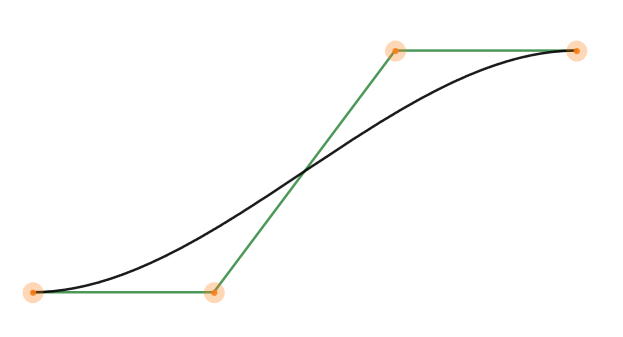
\includegraphics[width=0.8\textwidth]{../graphics/bezier_curve.png}
        \caption{Bezier Curve}
	\end{figure}
This is implemented in our code as follows:
\begin{lstlisting}
// p[4] are the four anchor points
static SDL_Point BezierPoint(float t, SDL_Point p[4]){
    float tt = t * t;
    float ttt = tt * t;
    float u = 1 - t;
    float uu = u * u;
    float uuu = uu * u;

	//returns a point on the curve for a certain value of t
    return (SDL_Point){
       uuu * p[0].x + 3 * uu * t * p[1].x + 3 * u * tt * p[2].x + ttt * p[3].x,
       uuu * p[0].y + 3 * uu * t * p[1].y + 3 * u * tt * p[2].y + ttt * p[3].y};
}
/* Changing the value of t from 0 to 1 in 100 steps will give 100 points on the curve. We can draw lines between consecutive points to get the desired curve.*/
\end{lstlisting}
The above function only returns one point which lies on the curve. Curve cannot be drawn based on a single point. So the following function is called which calculates a bunch of points along the curve and joins them with lines to draw a curve:
\begin{lstlisting}
static void DrawWire(SDL_Point start, SDL_Point end, bool hilo, bool simulating){
    /*
        This function draws a 3px thick bezier curve (the wire) between points start and end
        this is done by drawing 3 bezier curves next to each other
        hilo boolean represents what signal the wire is carrying (high or low)
        simulating boolean represents whether simulation is running or not
    */
    SDL_Point wirePoints[MAX_WIRE_PTS]; // array of points which will be joined to make the wire
    for (int i = 0; i < 3; i++){
        // to align the starting and ending points
        if (abs(start.x - end.x) > abs(start.y - end.y)){
            start.y++;
            end.y++;
        }
        else{
            start.x++;
            end.x++;
        }
        // anchor points between start and end
        SDL_Point p2 = {start.x + (end.x - start.x) / 3, start.y};
        SDL_Point p3 = {end.x - (end.x - start.x) / 3, end.y};
        // setting color of the wire
        // set red color if hilo is true and simulation is running 
        // set blue color if hilo is false and simulation is running 
        // set green color simulation is not running 
        if (i == 1){
            // to give bezier curve in the middle a lighter color
            if (hilo && simulating)
                SDL_SetRenderDrawColor(renderer, HIGH_COLOR, 255);
            else if (!hilo && simulating)
                SDL_SetRenderDrawColor(renderer, LOW_COLOR, 255);
            else
                SDL_SetRenderDrawColor(renderer, WIRE_NEUTRAL, 255);
        }
        else{
            // to give bezier curve in the middle a darker color
            if (hilo && simulating)
                SDL_SetRenderDrawColor(renderer, WIRE_HIGH_D, 255);
            else if (!hilo && simulating)
                SDL_SetRenderDrawColor(renderer, WIRE_LOW_D, 255);
            else
                SDL_SetRenderDrawColor(renderer, WIRE_NEUTRAL_D, 255);
        }
        // calculate all points along the curve
        for (int i = 0; i < MAX_WIRE_PTS; i++){
            float t = (float)i / MAX_WIRE_PTS;
            wirePoints[i] = BezierPoint(t, (SDL_Point[4]){start, p2, p3, end});
        }
        // make sure that wire touches starting and ending points
        wirePoints[0] = start;
        wirePoints[MAX_WIRE_PTS - 1] = end;
        // join all the points with lines
        SDL_RenderDrawLines(renderer, wirePoints, MAX_WIRE_PTS);
    }
}
\end{lstlisting}
    \section{Closing}
    Closing consists of destroying the textures and closing the libraries. This is done by following functions:
    \begin{lstlisting}
static void DestroyTextures()
{
    for (int i = 32; i < 127; i++)
        SDL_DestroyTexture(characters[i - 32]);
    for (int i = 0; i < 16; i++)
        SDL_DestroyTexture(displayChars[i]);
}

void CloseEverything()
{
    SDL_DestroyRenderer(renderer);
    SDL_DestroyWindow(window);
    DestroyTextures();
    SDL_Quit();
}
    \end{lstlisting}
\end{document}
